\section{Votación \onchain e incentivos}

Nebulas se dedica a la gobernanza \onchain y su compromiso es el de utilizar la tecnología \blockchain para proporcionar un entorno más abierto y colaborativo.

\subsection{Proceso de gobernanza \onchain}
\label{governance}

El proceso general de la gobernanza \onchain en Nebulas es como se describe a continuación:~\ref{fig:on-chain-governance}:

\begin{figure}
	\centering
	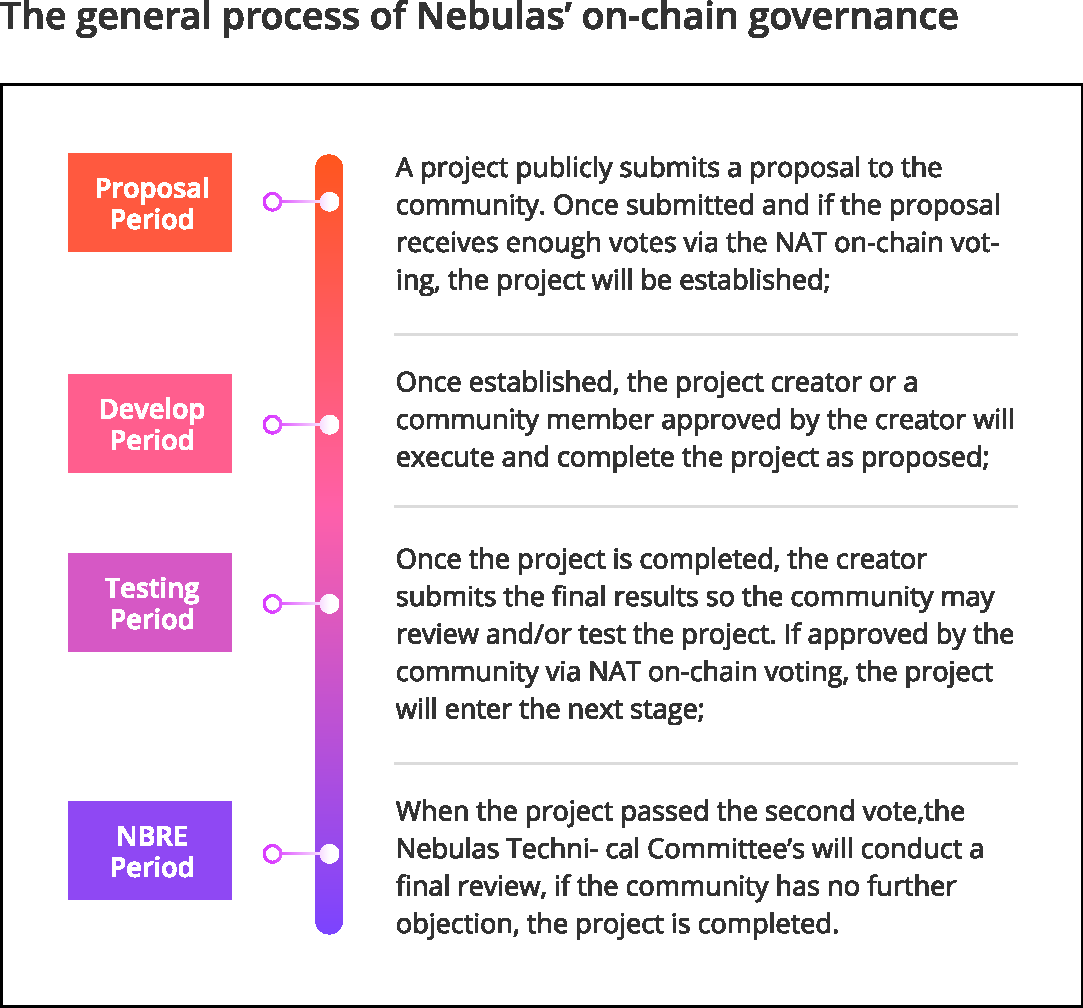
\includegraphics[width=1\textwidth]{../common/en/on-chain-governance.pdf}
	\caption{Proceso de gobernanza \onchain de Nebulas \label{fig:on-chain-governance}}
\end{figure}

\begin{enumerate}
	\item \textbf{Periodo de propuesta}: Se presenta públicamente una propuesta a la comunidad. Una vez presentada, y si la propuesta recibe suficientes votos a través de la votación NAT \onchain, se aprobará la ejecución del proyecto;
	\item \textbf{Periodo de desarrollo}: Una vez aprobado, el creador del proyecto —o el miembro de la comunidad aprobado por el creador— se encargará de ejecutar y completar el proyecto tal como se propuso;
	\item \textbf{Periodo de pruebas}: Una vez finalizado el proyecto, el creador enviará el resultado final para que la comunidad lo someta a revisión. Si la comunidad lo aprueba por medio del voto NAT \onchain, el proyecto pasará a la fase final;
	\item \textbf{Periodo \textit{NBRE}}: Cuando el proyecto pasa la segunda votación (revisión de la comunidad), el Comité Técnico de Nebulas realizará una revisión final. Si la comunidad no plantea ninguna objeción, el proyecto se marcará como completo.
\end{enumerate}

La gobernanza \onchain se basa en dos propiedades:

\begin{enumerate}
	\item La votación utiliza el token de gobernanza NAT y sus algoritmos subyacentes.
	\item El proceso de votación es bizantino, mediante tecnología \blockchain.
\end{enumerate}

Este Libro Naranja cubre principalmente los aspectos de la gobernanza \onchain.

\subsection{Principios básicos de votación}

El ecosistema de Nebulas integra las votaciones en su red principal. Cada voto emitido por los miembros de la comunidad es transparente y visible para todos. Dentro de Nebulas, la votación utiliza los siguientes principios básicos:

\begin{enumerate}
	\item La unidad básica de votación es una dirección \textit{mainnet} de Nebulas.
	\item El peso de los votos se referirá a la valuación de la dirección, dada por \nr.
	\item Las contribuciones positivas de los usuarios al sistema serán recompensadas con más derechos de voto. Creemos que la votación es una contribución positiva al ecosistema de Nebulas y que los usuarios deben estar motivados a recibir más derechos de voto.
\end{enumerate}

\subsection{Método de votación}

La votación será operada a través de un contrato inteligente en la red principal del \blockchain de Nebulas. Cada dirección podrá elegir entre tres opciones:

\begin{itemize}
	\item A favor
	\item En contra
	\item Abstención.
\end{itemize}

En forma adicional, los usuarios podrán decidir simplemente no ejercer su derecho a voto.

\subsection{El único medio utilizado para la votación: NAT}

\label{nat}

\subsubsection{Descripción general}

\begin{itemize}
	\item \textbf{Nombre}: Nebulas Autonomous Token
	\item \textbf{Símbolo bursátil (\textit{ticker})}: NAT
	\item \textbf{Estándar}: token NRC20
\end{itemize}

El Token Autónomo de Nebulas (\textit{Nebulas Autonomous Token, o NAT}) es un activo derivado de Nebulas Rank que se materializará en la forma de un token NRC-20, y que servirá como el único medio de voto dentro de la gobernanza del ecosistema Nebulas.

\begin{center}
	\fboxsep24pt
	\colorbox{yellow!30}{
	\begin{minipage}[c]{.8\textwidth}
		\paragraph{¿Qué es Nebulas Rank?}
		Nebulas Rank (NR) es el primer mecanismo nativo \onchain de medición de valor multidimensional de los datos \blockchain.

		Dentro de la economía de Nebulas, la unidad básica de gobernanza es una \emph{dirección}
		(\ref{rights}). Nebulas Rank cuantifica la contribución de cada
		\emph{individuo} a la acumulación económica por medio de la expresión matemática de la contribución de cada dirección. Nebulas Rank se divide en \emph{Core
		Nebulas Rank} y \emph{Extended Nebulas Rank}. Core Nebulas Rank refleja principalmente dos factores: el valor medio de una cuenta dentro de un período de tiempo determinado, y el grado de utilización de activos de esa cuenta durante un periodo de tiempo.

		A nivel macro, la relación entre el número de divisas, el valor del dinero, la tasa de circulación y la productividad dentro del \blockchain se puede describir con la ecuación clásica de la cantidad de dinero. El valor NR de la red entera refleja la liquidez total del ecosistema Nebulas, como así también su actividad.

		\paragraph{NAT y NR}

		La publicación de NAT se refiere principalmente a \emph{Core Nebulas Rank}, que muestra el rendimiento de los activos. En cada emisión semanal de NAT se revisará el valor NR con referencia al promedio y grado de utilización de los activos. Para más información en el sistema de valuación Nebulas Rank, sírvase consultar el \yellowp, publicado por el Instituto de Investigaciones de Nebulas en junio de 2018.

		\paragraph{¿Cómo se verifica mi valor Nebulas Rank?}

		Nebulas Rank, a través de Nebulas NOVA~\cite{nova} recibió su primera actualización el 6 de mayo de 2019. Esta actualización hizo uso del \textit{Nebulas Blockchain Runtime Environment (NBRE)} para lograr una actualización instantánea y autónoma. El algoritmo Nebulas Rank es de código abierto y se puede consultar en línea~\cite{CheckNR}.

	\end{minipage}}
\end{center}

\subsubsection{Casos de uso para el \textit{Nebulas Autonomous Token} (NAT)}

El token NAT es el único medio de voto válido en Nebulas. Los miembros de la comunidad pueden ejercer su voto \onchain mediante ese token y decidir la dirección que tomará el ecosistema de Nebulas; esas decisiones incluyen, pero no están limitadas, a:

\begin{itemize}
	\item la elección de los miembros del Concejo de Nebulas
	\item introducir ajustes al protocolo de Representación de Nebulas (\textit{Nebulas Protocol Representation, o NPR}) haciendo uso del Entorno Ejecutable Blockchain de Nebulas (\textit{Nebulas Blockchain Executable Environment, o NBRE}).
	\item establecer, votar y revisar propuestas comunitarias.
\end{itemize}

\subsubsection{Lanzamiento}

El método de distribución de NAT es similar al utilizado por Bitcoin —en cuanto existe un límite superior en el suministro total— y la cantidad distribuida semanalmente se irá decrementando.

El límite superior del suministro de tokens NAT está relacionado a la valuación \nr de la red mainnet en su conjunto. La cantidad emitida se decrementará semanalmente, con un coeficiente de atenuación de $\lambda$.

El valor inicial de $\lambda$ será de 0,997; esto significa que, por ejemplo, para la semana 180, la circulación se decrementará en un 58\% con respecto a la primera semana.

La circulación inicial de NAT dependerá del estado de la \mainnet de Nebulas NOVA luego de la finalización de su primera actualización de votación, programada para el 6 de mayo de 2019. Con base en la valuación \nr de la red completa, y de acuerdo a sus parámetros iniciales, el límite superior del total absoluto de NAT en existencia será de 100 000 000 000.

\subsubsection{Administración de los tokens NAT}

Los usuarios pueden administrar sus tokens NAT mediante la aplicación \textit{NAS nano Pro}~\cite{NASnano}, o cualquier otra cartera que dé soporte a tokens de estándar NRC20~\cite{wallets}. Los usuarios pueden ver las transacciones NAT y su circulación en cualquier explorador \blockchain de la mainnet de Nebulas~\cite{explorer}.

\subsection{Obtención de los tokens NAT}

Todos los usuarios que controlen al menos una dirección mainnet de Nebulas (exceptuando aquellas direcciones en lista negra) tendrán la oportunidad de recibir tokens NAT. Los propietarios de esas direcciones podrán obtener tokens NAT por medio de tres métodos:

\begin{itemize}
	\item mejorando la valuación NR de sus direcciones
	\item participando en las votaciones \onchain de Nebulas
	\item colocando NAS en prenda.
\end{itemize}

\paragraph{Direcciones NAT en lista negra}

Durante el proceso de distribución de los tokens NAT, cualquier dirección que entre en conflicto con uno o más los derechos básicos de las direcciones Nebulas (~\ref{rights}) ingresará automáticamente en una \textit{lista negra}.

Las direcciones en lista negra sólo podrán obtener tokens NAT si cumplen con sus derechos. Por ejemplo, la dirección (o direcciones) de una casa de cambio centralizada están en lista negra. De acuerdo al primer derecho básico, un propietario de direcciones Nebulas tiene el derecho de propiedad y uso de sus activos en Nebulas; así, la dirección de la casa de cambio podría obtener NAT de acuerdo a su valuación NR y bajo las mismas condiciones que otros usuarios. No obstante, la propiedad (es decir, los tokens NAT) de la casa de cambio deberían ser distribuidos a sus correspondientes usuarios. De acuerdo a los derechos básicos restantes, la dirección de la casa de cambio no posee derecho a iniciar una propuesta o a participar en votaciones a menos que la casa de cambio demuestre que los activos de esa dirección representan plenamente la propuesta de un usuario o su disposición para votar. De ese modo, las direcciones en lista negra no pueden obtener incentivos NAT mediante participación en votaciones.

\subsubsection{Recepción de tokens NAT mediante la mejora de la valuación NR de una dirección}

Los tokens NAT se distribuirán semanalmente a las distintas direcciones \textit{mainnet} de Nebulas cuya valuación NR sea positiva. El número de tokens NAT distribuidos estará basado en el valor semanal NR de la dirección, y del NR de la red en su conjunto.

El número de tokens distribuidos se decrementará semanalmente. El coeficiente de atenuación es $\lambda$. Inicialmente, $\lambda$ = 0,997.

En la $i$a semana, la proporción será:

\begin{align}
1\,\text{NR}=z(x_{ne},x_{e},\mu)\times\lambda^{i}\,\text{NAT}
\end{align}

Descripción de la fórmula anterior:

\begin{itemize}
	\item $\lambda$: coeficiente de atenuación.
	\item $\mu$: parámetros del incentivo de comportamiento de voto.
	\item $x_{ne}$: la suma de la valuación NR de las direcciones de la mainnet en su conjunto (excepto casas de cambio centralizadas).
	\item $x_{e}$: la suma de la valuación NR de la mainnet en su conjunto.
	\item $z(x_{ne},x_{e},\mu)$: función con $x_{ne}$, $x_{e}$ y $\mu$ como variables, Nebulas Rank y proporción de pago de NAT.
\end{itemize}

\subsubsection{Prendar NAS para recibir NAT}

Comenzando a partir del 6 de mayo de 2019, los usuarios de la mainnet de Nebulas podrán optar por recibir NAT \emph{prendando} la criptodivisa nativa de Nebulas, NAS, a través de un contrato inteligente.

El usuario de ese contrato inteligente recibirá tokens NAT a partir de la segunda semana luego de haber realizado la prenda. Si el usuario cancela la prenda, la distribución de tokens NAT cesará de inmediato.

El número de tokens distribuidos semanalmente se irá decrementando de acuerdo a un coeficiente de atenuación $\lambda$. Inicialmente, $\lambda$ = 0,997.

La proporción de NAT a recibir por NAS prendados, durante la $i$a semana:

\begin{align}
x\,\text{NAS} \rightarrow \alpha \times z(x_{ne},x_{e},\mu)\times g(x) \times
  \lambda^{i}\,\text{NAT}
\end{align}

Descripción de la fórmula:

\begin{itemize}
	\item $x$: NAS prendados.
	\item $\alpha$: coeficiente de prendado, $\alpha$=5 en el estado inicial.
	\item $z(x_{ne},x_{e},\mu)$: función con $x_{ne}$, $x_{e}$, y $\mu$ como variables, la proporción de intercambio de NR y NAT.
	\item $g(x)$: una función asociada con $x$ que simula la valuación NR obtenida por los NAS $x$ de la mainnet de Nebulas.
\end{itemize}

\paragraph{¿Cómo se inicia la prenda de NAS?}
Para iniciar el proceso, los usuarios deben enviar una transacción al contrato inteligente correspondiente, mediante una cartera Nebulas (tal como la NAS nano Pro). Al hacerlo, los NAS prendados quedarán bloqueados en el contrato inteligente hasta que el usuario decida cancelar la prenda.

Para garantizar la adquisición de tokens NAT, el usuario debe enviar sus NAS al contrato inteligente (\textit{Pledge smart contract}) a través de una dirección controlada por el usuario, y de la cual posea su clave privada. Los usuarios no deben, bajo ninguna circunstancia, enviar NAS al contrato inteligente desde una casa de cambio o desde una dirección sobre la cual no tengan la clave privada.

\paragraph{¿Cómo se cancela el contrato de prenda?}

Si el usuario decide cancelar la prenda y desbloquear sus NAS, cualquier cartera NAS con soporte a contratos inteligentes y tokens NRC-20 podrá interactuar con el contrato inteligente previamente mencionado para cancelar la prenda. Luego de cancelarla, los NAS previamente prendados quedarán desbloqueados y a disposición del usuario.

\subsubsection{Recepción de NAT por medio del voto \onchain en Nebulas}

La recepción de tokens NAT se llevará a cabo al comienzo de cada semana dentro de la mainnet de Nebulas. Una vez que las direcciones reciban sus NAT, pueden utilizarlos para votar en distintas elecciones y proyectos. Las opciones de voto son \textit{For} (a favor), \textit{Against} (en contra), or \textit{Abstain} (abstención); cada elección es una opción válida para recibir incentivos. Si el usuario no participa en ninguna votación durante el ciclo semanal, no recibirá ningún incentivo semanal la semana siguiente.

\paragraph{Proporción de incentivos}

La distribución y proporción de los incentivos debe ser justa y no utilizarse maliciosamente. Para cumplir con esos requisitos, la distribución semanal de tokens NAT tendrá en cuenta lo siguiente:

\begin{enumerate}
	\item El número de tokens NAT que la dirección dada utilizó para votar durante la semana.
	\item La cantidad de tokens NAT recibidos en la semana en relación a la valuación NR de la semana previa.
\end{enumerate}

Si una persona utiliza para votar una cantidad de NAT menor o igual al total recibido de acuerdo a su valuación NR, los NAT utilizados serán tenidos en cuenta en el algoritmo de incentivos; si esa persona utiliza una cantidad de NAT superior a la correspondiente a su valuación NR, esa parte no será tenida en cuenta por el algoritmo de incentivos.

Durante la $i$a semana, la distribución de incentivos NAT en cada dirección mainnet utilizará la siguiente fórmula:

\begin{align}
\mu \times \min \{N_{v}, N_{nr}\} \times \lambda^{i}
\end{align}

\begin{itemize}
	\item $\mu$: parámetros de los incentivos, $\mu$=10 bajo los parámetros iniciales.
	\item $\lambda$: coeficiente de atenuación, valor $\lambda$=0,997.
	\item $N_{v}$: la cantidad de NAT utilizados para votar la semana previa.
	\item $N_{nr}$: cuántos NAT recibirá la dirección esa semana de acuerdo a su valuación NR en la semana previa.
\end{itemize}

\noindent Cuando $N_{v}$ (enviados por la dirección durante la semana) es menor o igual a $N_{nr}$, el número de incentivos NAT obtenidos será de $\mu\times N_{v}$. Cuando la $N_{v}$ de la dirección es mayor a $N_{nr}$, la cantidad de incentivos será de $\mu\times N_{nr}$.

\paragraph{Ejemplo}

Una dirección obtiene 10 NAT de acuerdo a la valuación NR de la semana previa. Esa dirección guarda 1000 NAT adicionales.

Esa semana la dirección utiliza 5 NAT en votaciones, lo cual es menor a los 10 NAT recibidos por su valuación NR de la semana anterior; como recompensa, recibirá $10\times5=50$ NAT en incentivos de voto.

Si la dirección decide utilizar 1000 NAT para votar, lo cual excede los 10 NAT recibidos por la valuación NR de la semana previa, recibirá $10\times10=100$ NAT como incentivos de voto.

\paragraph{}

En forma similar a lo anterior, la distribución del incentivo NAT también se decrementará semanalmente por el mismo coeficiente. Bajo los parámetros iniciales, $\lambda$, el coeficiente de atenuación será $\lambda$=0,997.

\subsection{Reglas de voto}

\subsubsection{Tarifa de votación}

Cada voto costará $\theta$\% NAT como tarifa de votación, lo cual está autorizado por el Concejo de Nebulas, para ser administrado por la Fundación Nebulas como un fondo especial de operaciones para el proyecto NAT. El equipo del citado proyecto no podrá usar los NAT así recolectados para votar. El valor inicial de la tarifa de voto es $\theta$=3.

\subsubsection{Votación y destrucción de los tokens NAT}

Durante cada ciclo semanal de emisión, los NAT que los usuarios utilicen en la mainnet de Nebulas, por medio del contrato inteligente, serán destruidos inmediatamente. No obstante ello, también se distribuirán nuevos tokens NAT de forma semanal por los métodos descriptos más arriba, con el fin de reducir la tasa de destrucción global. La proporción de tokens destruidos se irá decrementando de acuerdo al ciclo. La tasa de desaceleración es consistente con la tasa de emisión. La cantidad de NAT a destruir durante cada ciclo será calculada de acuerdo a la función que se provee en el anexo; véase ref{burn}.

\subsubsection{Requerimientos de aprobación de las votaciones}

Para que una propuesta sea aprobada, los votos deben reunir dos criterios: grado de participación en la votación, y proporción de votos a favor.

\begin{enumerate}
	\item

	\textbf{Participación:}

	Para aquellas propuestas que involucren el uso de activos públicos, la cantidad total de votos no debe ser menor que la proporción de activos requeridos por la propuesta en relación al total de activos en circulación en la mainnet.

	Si una propuesta requiere el uso de $X$ NAS, y la cantidad de NAS en circulación dentro de la mainnet (cualquier NAS que no está bloqueado o prendado, y que está disponible para su transferencia inmediata) es de $Y$, la propuesta debe alcanzar una tasa de participación no menor a
	$X/Y$, que se convierte en NAT; la proporción de los NAT participantes en la votación no deben ser menor a $X/Y$.

	Para aquellas propuestas que no requieren el uso de activos públicos, la participación será determinada por la comunidad. Tales propuestas incluyen, pero no se limitan, a: ajuste de los parámetros de la mainnet, un NPR a ser ejecutado por la NBRE, etcétera.

	\item

	\textbf{Proporción de votos a favor:}

	Adicionalmente al requerimiento de participación mínima, la proporción de votos positivos requerida en una votación en particular debe alcanzar o superar el 51\%.
	Dicho de otro modo: asumiendo que una propuesta recibe un total de $X$ votos, de los cuales el total de votos afirmativos es $S$, el total de votos negativos es $N$ y los votos en abstención se representan por $A$, la propuesta se considera aprobada si $S/(S+N+A) \ge 51\%$.

\end{enumerate}

\subsection{Supervisión y administración de las votaciones}

\subsubsection{Supervisión del proceso de votación}
\label{second-vote}

El Comité Técnico es nombrado por el Concejo para supervisar el proceso de gobernanza y asegurar que todo el proceso sea abierto y transparente. La votación pública sobre el \blockchain de Nebulas está organizada y administrada por el Comité Técnico.

Toda votación pública admite la supervisión por parte de cualquier miembro de la comunidad. Ante aquellas propuestas que violen cualquier derecho básico de una dirección de Nebulas, el Comité Técnico podrá solicitar su revisión al Concejo. Como supervisor de la legitimidad del proceso de gobernanza dentro del ecosistema de Nebulas, el Concejo tiene el derecho de presentar una y sólo una solicitud para un \textbf{segundo voto}.

Cuando el Concejo solicita una \textbf{segunda votación}, se considera que la propuesta ha entrado en un nuevo ciclo de votación, por lo cual no se ejecutan los resultados de la primera votación. El NAT utilizado en la votación del ciclo inicial no será devuelto y será quemado de acuerdo a la tasa de quemado del ciclo semanal en vigencia.

La participación en la segunda votación debe ser mayor que la participación en la primera. Es decir, si el grado de participación de la primera votación es de $X/Y$, el grado de participación de la segunda votación deberá ser superior a $X/Y$, y la proporción de votos a favor no deberá ser inferior al 51\%.

\subsubsection{Parámetros de ajuste para NAT}

El proceso de distribución de tokens NAT involucra los siguientes factores:

\begin{enumerate}
	\item $\alpha$: coeficiente de prenda, valor inicial $\alpha$=5
	\item $\mu$: factor de recompensa de voto, valor inicial $\mu$=10
	\item $\lambda$: coeficiente de atenuación, valor inicial $\lambda$=0,997
	\item $\theta$: tarifa de votación, valor inicial $\theta$=3
\end{enumerate}

El ajuste del coeficiente se debe realizar a través del sistema de gobernanza por voto; la Fundación Nebulas o el equipo del proyecto NAT no tienen derecho a ajustar los coeficientes sin autorización de la comunidad.